\documentclass[twoside,a4paper]{refart}

\usepackage{newunicodechar} %greek letters

\usepackage{makeidx}
\usepackage{ifthen}
\usepackage{graphicx}
\graphicspath{{figures/}}
\usepackage{float}
\usepackage{hyperref}
\usepackage{cleveref}
\usepackage[acronym,nomain,nonumberlist]{glossaries}
\usepackage{soul}

\usepackage{url}

\author{Miguel Sim\~ao (miguel.simao@uc.pt) \\
		\ \\
		Collaborative Robotics Group \\
		Department of Mechanical Engineering \\
		University of Coimbra}
\title{Reference Manual for the Implementation of the Control System for a Pneumatic Valve over the TCP/IP Protocol}
\date{}
\emergencystretch1em  %

\pagestyle{myfootings}
\markboth{Pneumatic valve control over network}%
		 {Pneumatic valve control over network}

\makeindex 

%from glossaries package
\makeglossaries
\newacronym{gpio}{GPIO}{General Purpose Input/Output (Raspberry Pi)}
\newacronym{rpi}{RPi}{Raspberry Pi}
\newacronym{no}{NO}{Normally Open}
\newacronym{nc}{NC}{Normally Closed}


\setcounter{tocdepth}{2}

\begin{document}
	
\maketitle


\begin{abstract}
	Documentation for the set up that actuates a pneumatic valve at the base of the IIWA. The end goal is to commutate air pressure between the two air inputs according to a control message to be sent over a TCP/IP socket. On the first section, we show how the current set up can be used and a list of things that may be implemented in a future version. The second section describes in detail the hardware used in each of the subsystem of the system. The last section concerns both the network configuration and software used on the controller. It also describes how the system can be replicated, updated and extended.
\end{abstract}

\tableofcontents

\newpage

% \glsaddall
% \printglossary[type=\acronymtype,title=Acronyms]



%%%%%%%%%%%%%%%%%%%%%%%%%%%%%%%%%%%%%%%%%%%%%%%%%%%%%%%%%%%%%%%%%%%%

\section{Introduction}
\subsection{Usage}
The RPi server accepts several connections over the TCP/IP protocol, for which you need to provide an IP address and a port. As of now, the RPi has a static IP address in the wi-fi network that you should only use if you're trying to connect over wi-fi:
\begin{verbatim} 192.168.1.199 \end{verbatim}
This IP should be valid forever. The port used is 1080. If you're trying to connect from a computer in the lab's wired network, the temporary IP address you should use is (Ethernet):
\begin{verbatim} 172.16.22.197 \end{verbatim}
at the same port. This is the IP of the router in the department's network and it will redirect the connection to the target RPi only if you use port 1080. Otherwise, you have to change some network configurations.\seealso{See \Cref{sub:network_conf}}. \attention For now, the IP address of the router is dynamic, but it will be given a static IP to be defined in the close future.

You also have the option to connect directly from the Ethernet port. For this end, the IP address is 172.31.1.1 and the port is the same (1080). This is useful if you're trying to connect from the robot's local network (172.31.x.x).

You can turn on the RPi just by powering it with a \mu USB cable. The server is running when the large red LED is bright. The following commands are available:
\begin{enumerate}
	\item
	O10 - [Default] Turns on "Air 1" and locks tool
	\item
	O11 - Turns on "Air 2" and unlocks tool
	\item
	reboot - reboots the RPi
	\item
	shutdown - shuts down the RPi
\end{enumerate}
Every command should include a terminator that is CR/LF (carriage return and line feed). The first character of the output is the letter "O", for Output. The next character is the output number, which at this time is just the "1". The final character sets the value ON ("1") or OFF ("0") of the digital output @24VDC. 

\subsection{Matlab Example}
This example requires Matlab and the Instrument Control Toolbox to create the TCP/IP connection.
The process to set up the TCP/IP connection and control the locking/unlocking of the robot's tools is simple:
\begin{enumerate}
	\item Create connection object
	\item Set connection properties
	\item Open connection
	\item Send commands
	\item Close connection
\end{enumerate}
This is valid for most languages. Specifically for Matlab, we can do:
\begin{verbatim}
% Instantiate 'tcpip' object:
t = tcpip('192.168.1.199',1080)
% Set terminator (non-default):
t.Terminator = 'CR/LF';
% Open connection:
fopen(t)
% Send command (unlock):
fprintf(t,'O11');
% Send command (lock):
fprintf(t,'O10');
% Close connection:
fclose(t)
\end{verbatim}


\subsection{"To do" List}
List of things to implement on the future:
\begin{enumerate}
	\item
	\marginlabel{LOW PRIORITY} Maybe change to a connectionless type of sockets ({\tt SOCK\_DGRAM})
	\item
	\marginlabel{MEDIUM PRIORITY} Implement ACPI to the RPi to prevent damage
	\item
	\marginlabel{HIGH PRIORITY} Add a manual override to the valve control (lock/unlock)
	\item
	\marginlabel{HIGH PRIORITY} \st{Configure RPi to connect to the local network of the robot through its Ethernet port}
\end{enumerate}

\section{Hardware}
In this section we describe the different subsystems that can be defined in this system. We also describe their purpose and the relationships between distinct subsystems. To get an overview of the whole system, please check \cref{sub:hardware:full}.

\subsection{Material List}

To begin with, you have access to the following parts:
\begin{enumerate}
	
\item
Pneumatic valve with electric control
\item
24VDC power supply
\item
Relay board (breakout)
\item
5VDC regulated power supply
A regular USB power supply of at least 2.5A suffices. 
\item
Raspberry Pi 2
\item
USB Wi-fi adapter
\item
1 Red LED
\item
1 100\Omega \ resistor
\item
2 Yellow LEDs
\item
2 1500\Omega \ resistors
	
\end{enumerate}

\subsection{Actuation Subsystem}\label{sub:actuation_system}
The actuation subsystem is composed by the commutation pneumatic valve. As the system is currently set up, the Air 1 output at the flange also feeds the tool itself (e.g.: gripper). So, if you unlock the tool, it is going to lose the air pressure.

The actuation subsystem interfaces with the control subsystem. It moves the valve between the following two positions:

\begin{enumerate}
	\item
	\marginlabel{Ouputs:}
	P2 -- Pneumatic output 2
	\item
	P4 -- Pneumatic output 4 
\end{enumerate}

It requires as input the 24 VDC signals and a GND connection (referenced to the input signals):
\begin{enumerate}
	\item
	\marginlabel{Inputs:}
	S1 -- 24V signal 1 (S1)
	\item
	S2 -- 24V signal 2 (S2)
	\item
	GND24 -- Ground
\end{enumerate}
The input signal S1 activates P2 and S2 activates P4.

\marginlabel{When you turn on the system, Air 1 is active and locking the tool.}
A real representation in shown in \cref{fig:ph_actuation}. In this figure, P1 is the pressured air input from its source, P3 and P5 are sinks, P12 and P14 are connected with P1 and assist the actuation of the valve. P2 is connected to {\tt Air 1} to the robot and P4 to {\tt Air 2}. When the system is on, {\tt Air 1} is the normally pressured line. If the system is off, both air line are locked.

\begin{figure}[H]
	\centering
	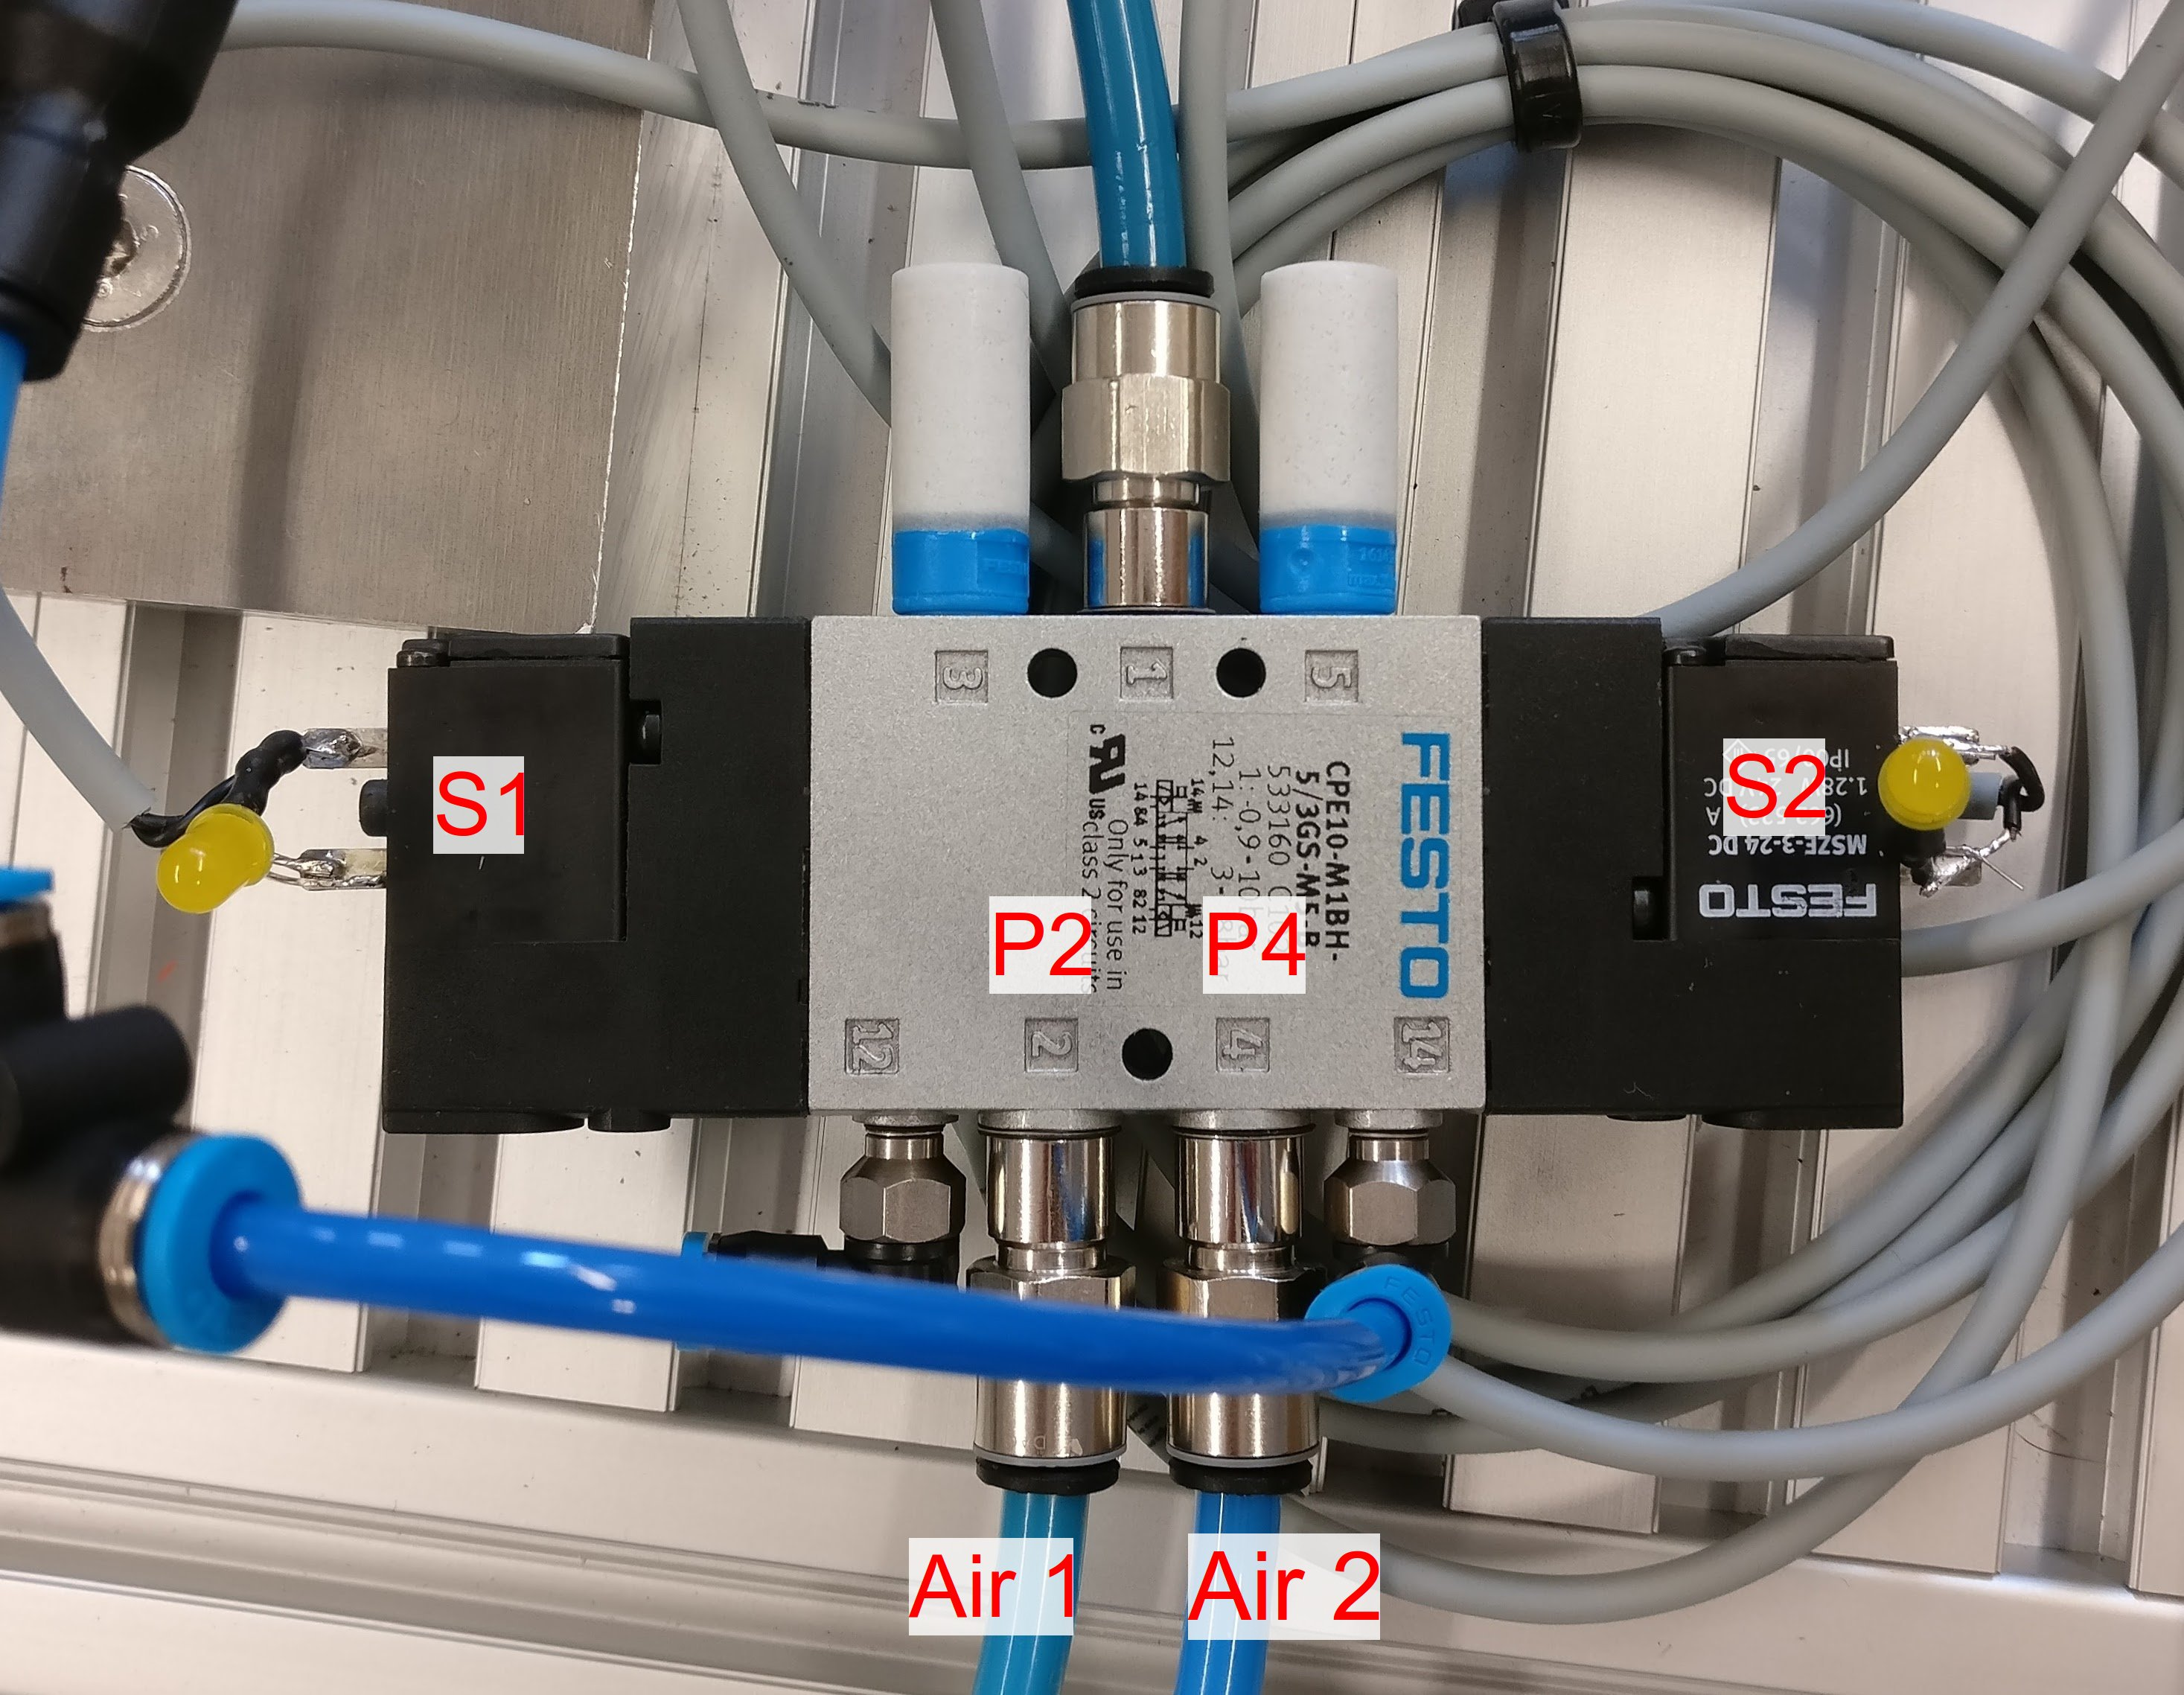
\includegraphics[width=1.0\linewidth]{ph_actuation}
	\caption{Actuation subsystem. Pneumatic valve with 3 positions and electrically-assisted control.}
	\label{fig:ph_actuation}
\end{figure}

\subsection{Control Subsystem}
The control subsystem is composed of the relay and interfaces with the communications subsystem and the actuation subsystem.

\seealso{See \Cref{sub:actuation_system}} The actuation valve is normally centred and requires two 24V signals to commutate between P2 and P4 (see \cref{sub:actuation_system}). To provide those, we use a single relay (\cref{fig:relay_0}) to commutate a 24V source from a power supply, between the two signals S1 and S2. The control signal should be 5V but can be done with the 3.3V output level of the RPi.

\begin{figure}[H]
	\centering
	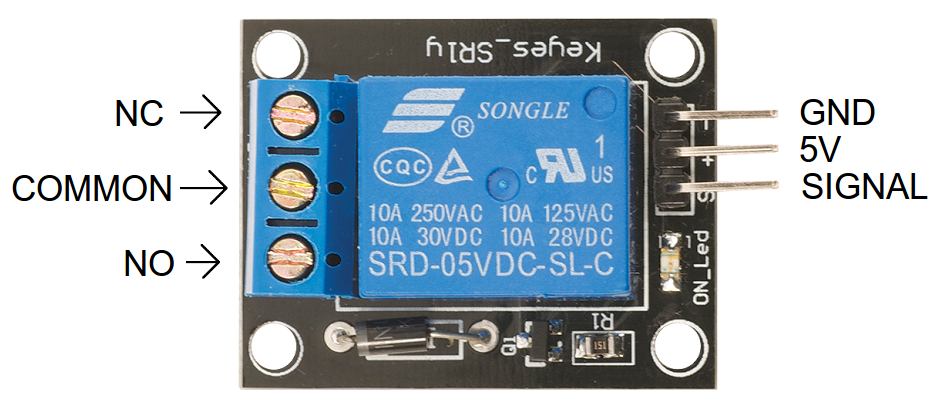
\includegraphics[width=0.7\linewidth]{relay_0}
	\caption{Board with one relay. NC stands for normally closed and NO for normally open.}
	\label{fig:relay_0}
\end{figure}

When the RPi digital output is high (3.3V), the relay connects (left side of the picture) the common line to the \gls{no} line. Otherwise, the \gls{nc} line is active.
The 5V (DC) input may come from the RPi 5V line and GND from the GND line on the RPi's \gls{gpio} pins.

\begin{enumerate}
	\item
	\marginlabel{Outputs:}
	S1 -- 24V signal 1 (S1)
	\item
	S2 -- 24V signal 2 (S2)
\end{enumerate}

\begin{enumerate}
	\item
	\marginlabel{Inputs:} S -- Control signal (3.3V)
	\item PWR24 -- 24 VDC from source
	\item PWR5 -- 5 VDC from source
	\item GND5 -- Ground referenced to PWR5
\end{enumerate}

\begin{figure}[H]
	\centering
	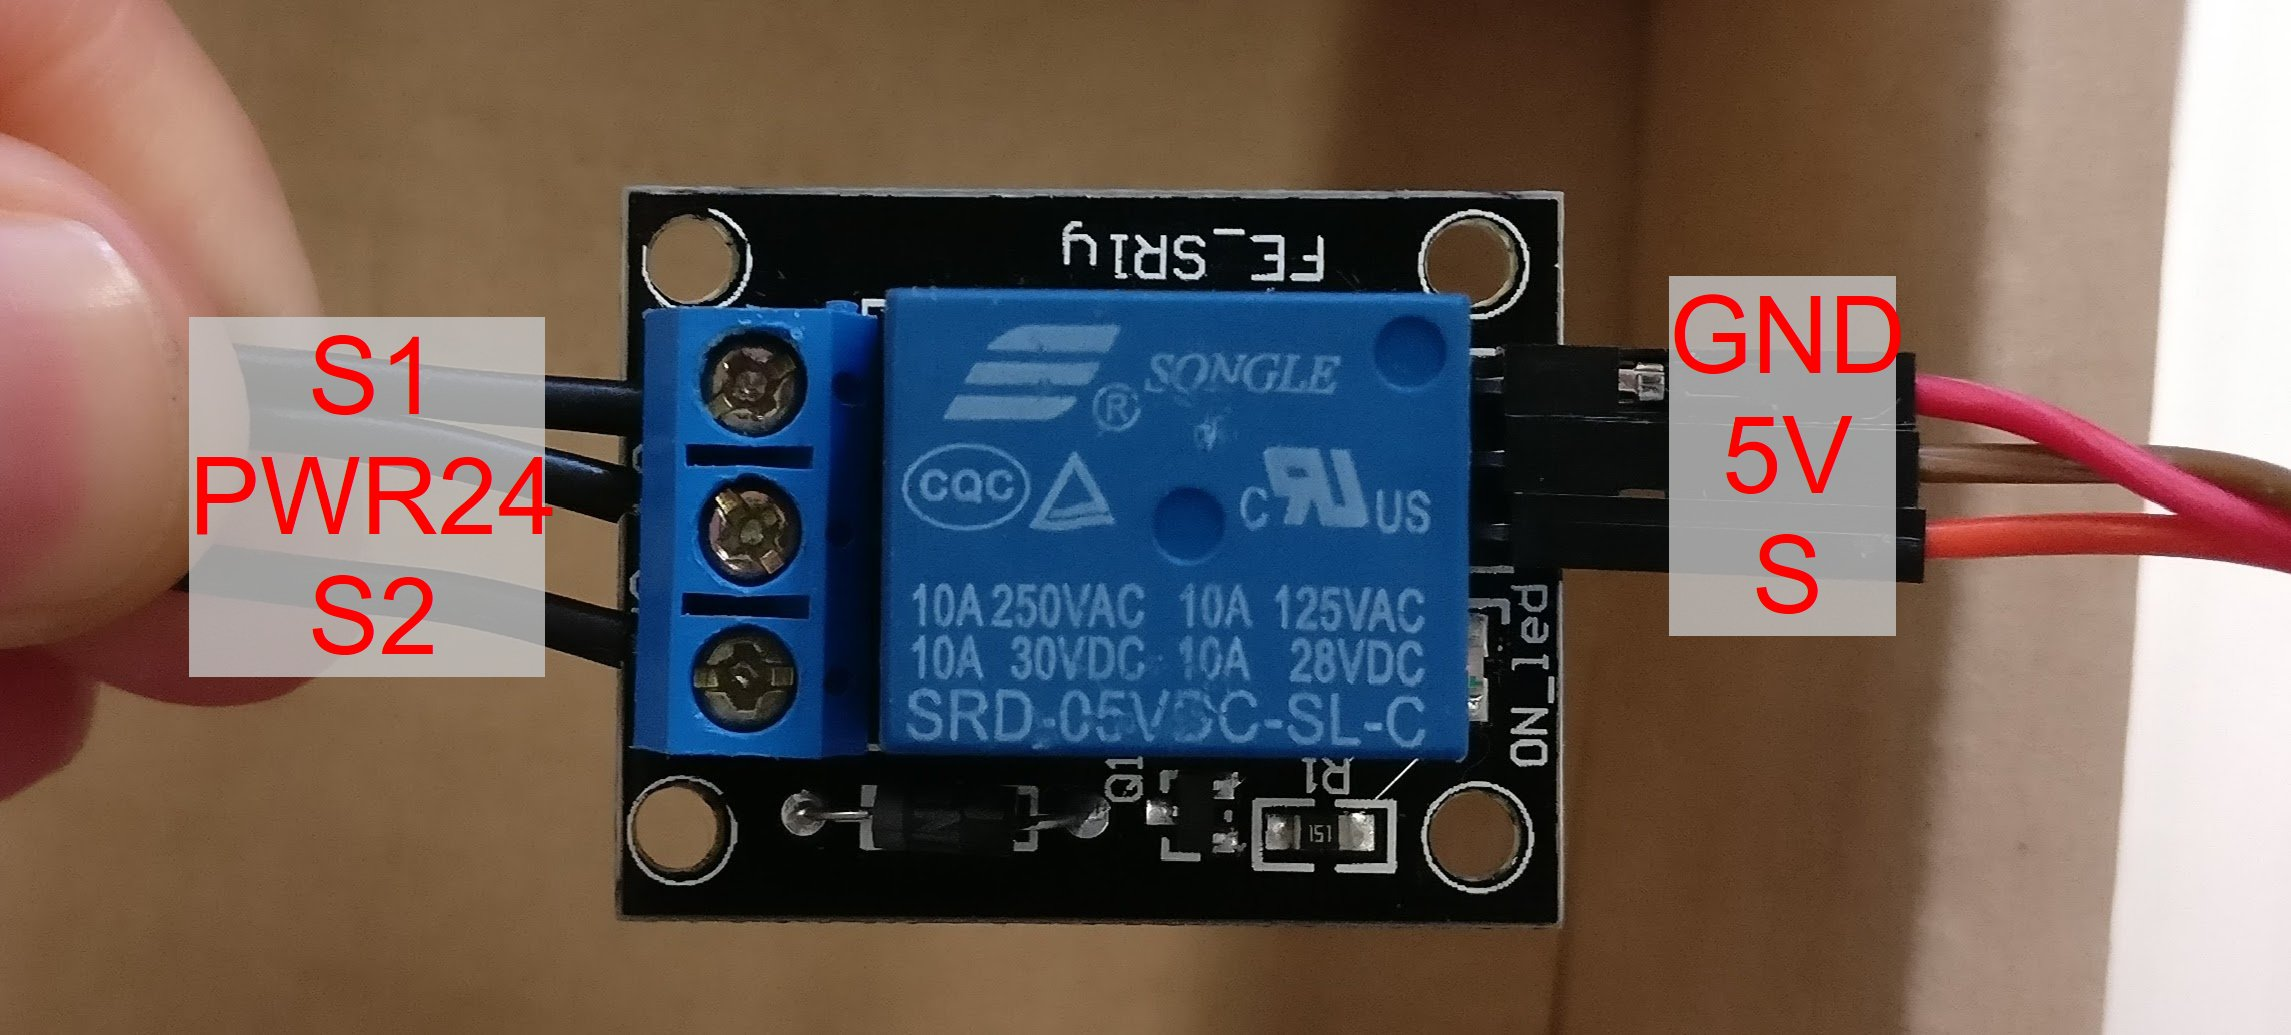
\includegraphics[width=1.0\linewidth]{ph_control}
	\caption{Control subsystem. Single relay board with 24V rail on the left side and the control side on the right.}
	\label{fig:ph_control}
\end{figure}

\subsection{Communications Subsystem}
The communications subsystem is a Raspberry Pi with a socket server running that allows remote connections. It is composed by the RPi (\cref{fig:ph_com}) and an USB Wi-fi adapter OR an Ethernet connection. Both interfaces can also be connected (Ethernet + Wi-fi). For reference, the \gls{gpio} pin layout is shown in \cref{fig:rpi2_gpio}.

\seealso{See \Cref{fig:rpi2_gpio} to see GPIO header pin layout.}A real representation of the subsystem in shown in \cref{fig:ph_com}. Power to the RPi is provided by the \mu USB input, but it is also possible to power it from a regulated\footnote{Careful! There's no circuit protection on the GPIO header, so if your supply peaks above 5V, you can fry your RPi.} 5V power supply to pin 2. Regarding outputs, power and ground to the control subsystem are derived from the 5V output at pin 4 and 6. The control signal {\tt S} is provided by pin 7 (GPIO4). There's also a red indication LED connected to pins 26 (anode) and 25 (cathode).



Input/output list:
\begin{enumerate}
	\item  \marginlabel{Ouputs:} S -- Control signal for the control subsystem
	\item PWR5 -- 5VDC (limited amperage)
	\item GND5
\end{enumerate}
\begin{enumerate}
	\item  \marginlabel{Inputs:} Network (USB Wi-fi or Ethernet)
	\item PWR5 -- 5VDC from source or USB
	\item (Optional) GND5 -- Ground, if USB is NOT used
\end{enumerate}

\begin{figure}[H]
	\centering
	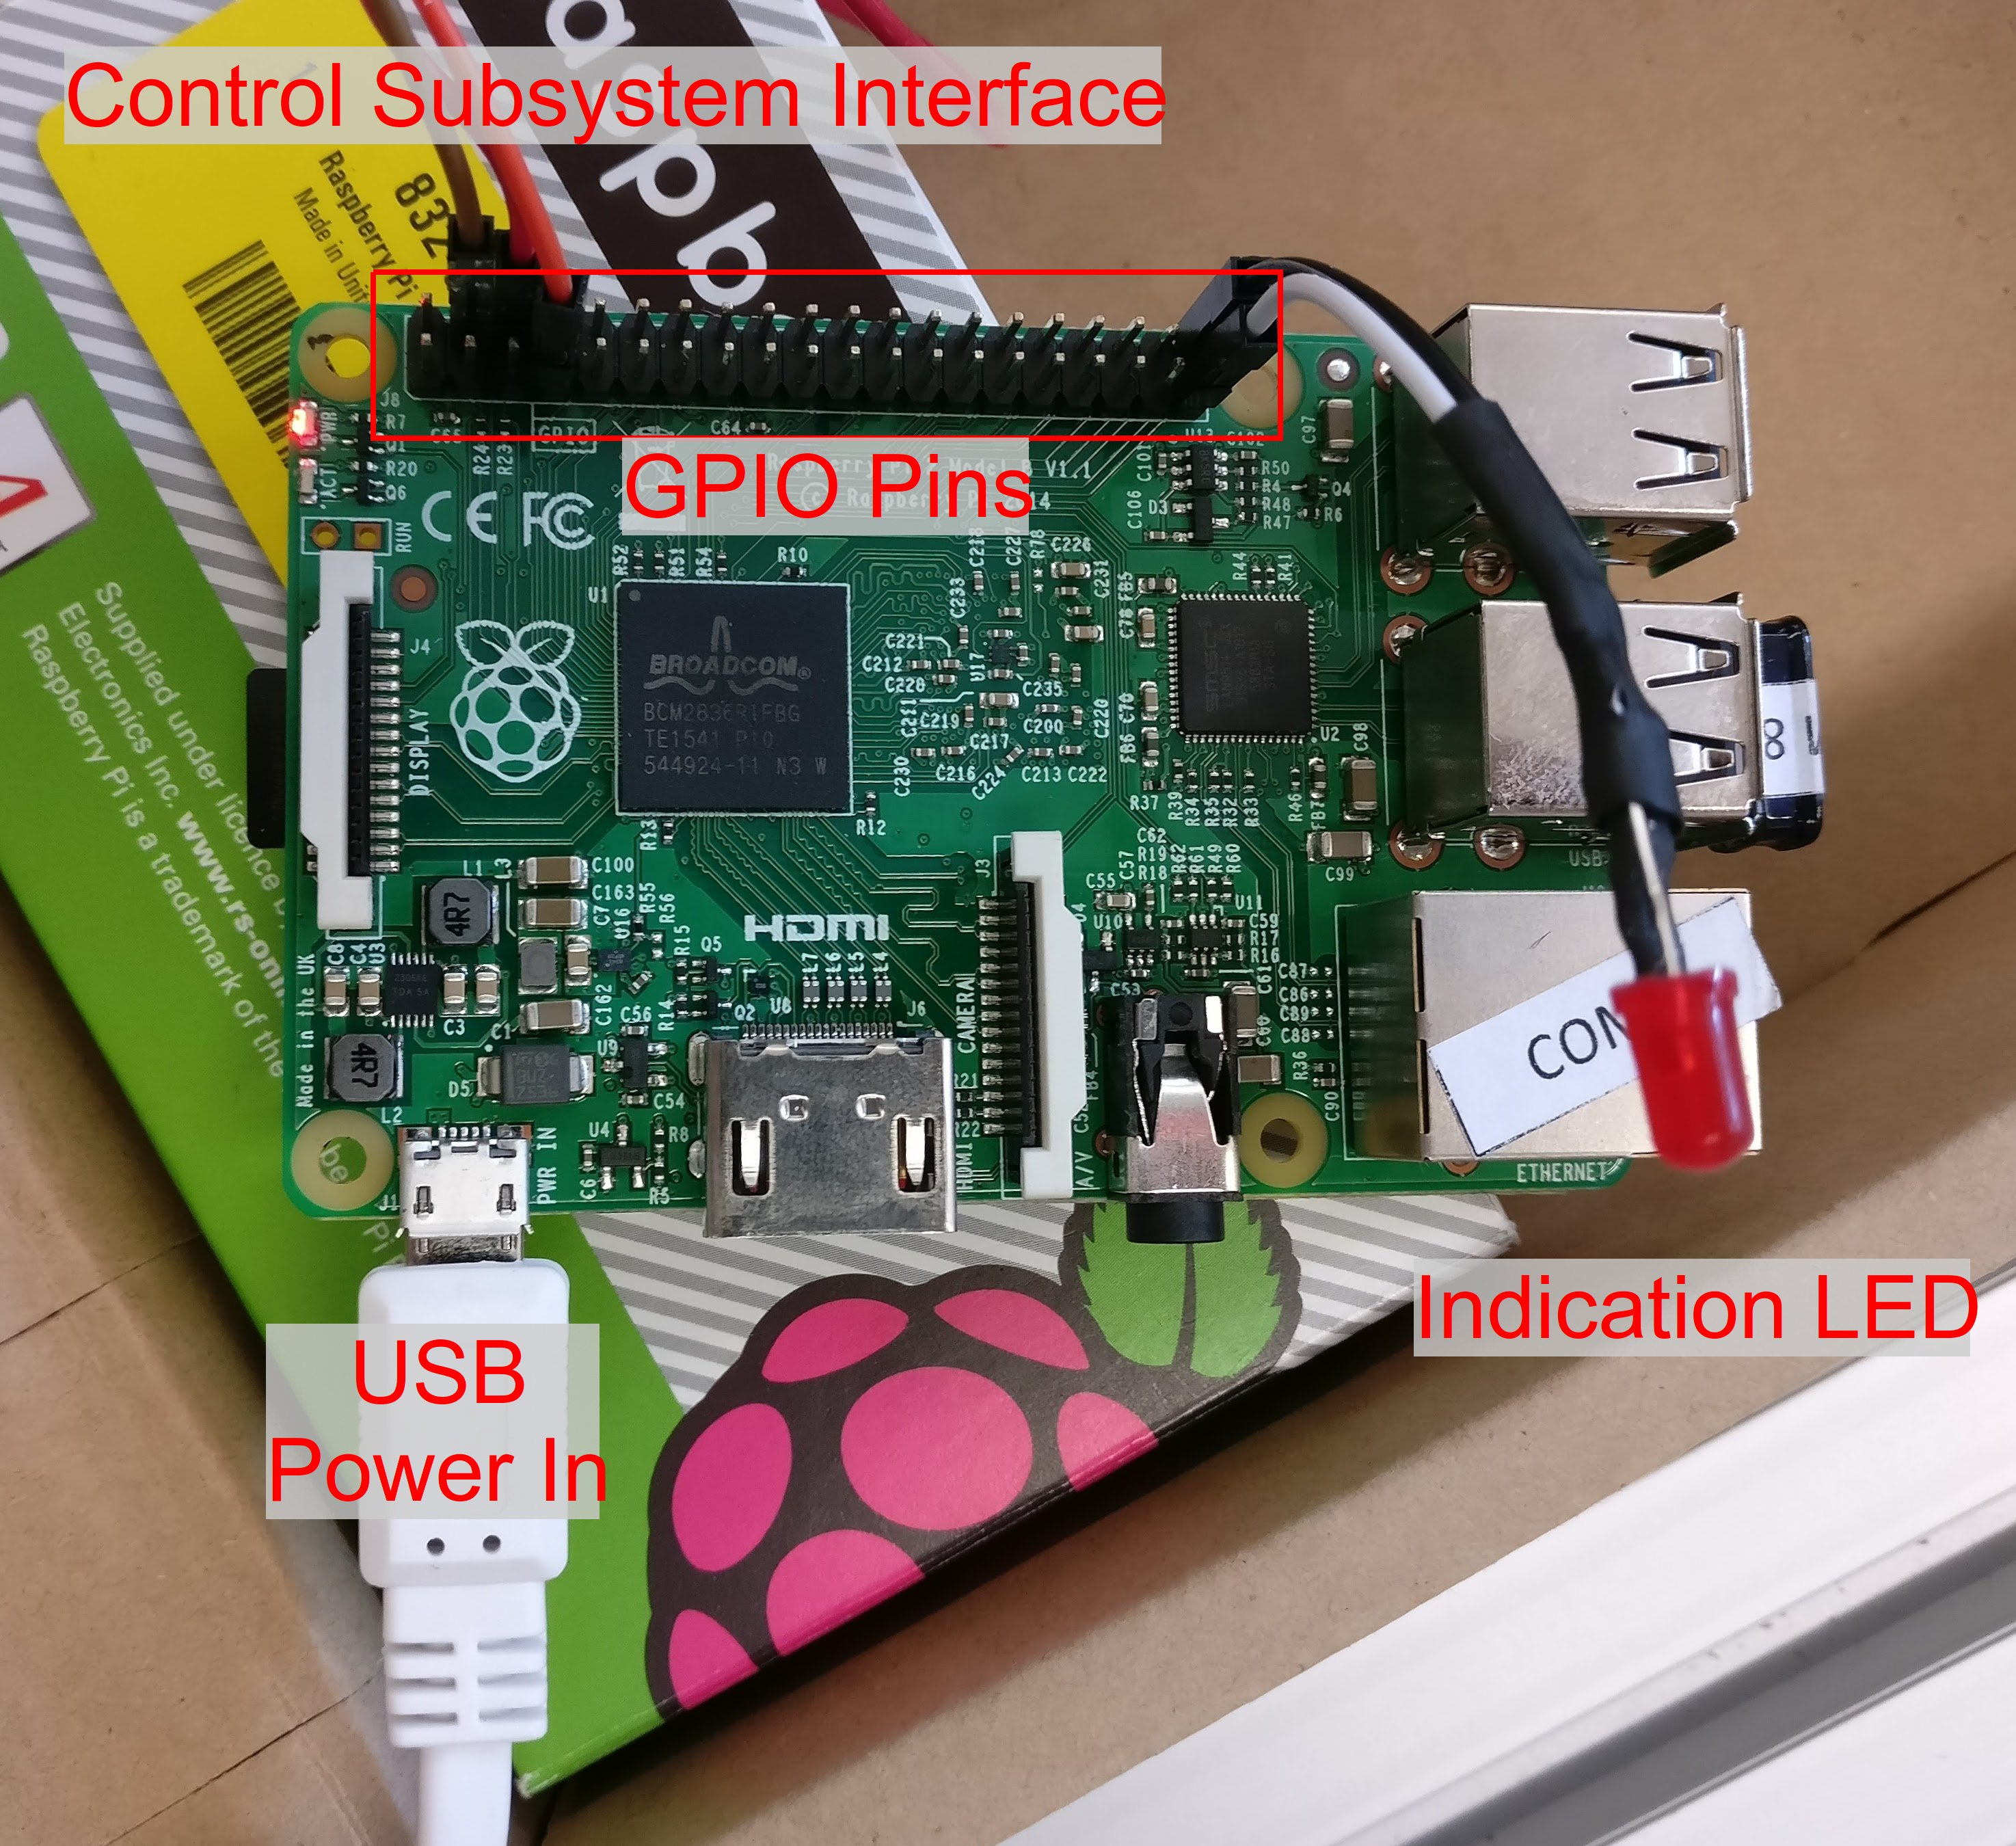
\includegraphics[width=1.0\linewidth]{ph_com}
	\caption{Real set-up of the communications subsystem.}
	\label{fig:ph_com}
\end{figure}

\begin{figure}[H]
	\centering
	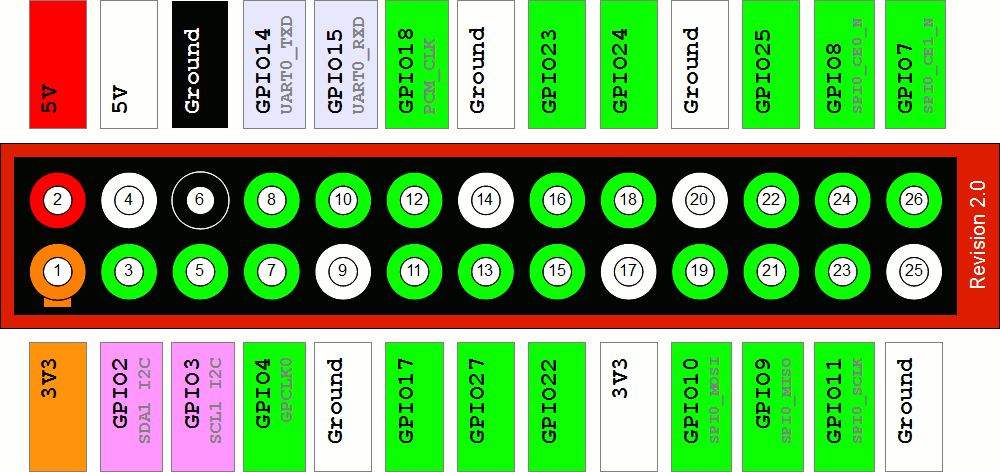
\includegraphics[width=1.0\linewidth]{rpi2_gpio}
	\caption{Raspberry Pi 2/3 \gls{gpio} layout.}
	\label{fig:rpi2_gpio}
\end{figure}

\subsection{Power Subsytem}
There are two power rails in this system: 24 VDC and 5 VDC. There are separate power supplies for each, so the grounds are referenced individually. The 5 VDC supply is required for the Raspberry Pi and the control subsystem.
\begin{enumerate}
	\item  \marginlabel{Ouputs:} PWR24 -- 24 VDC source
	\item GND24 -- Ground for 24 VDC devices
	\item PWR5 -- 5 VDC source
	\item GND5 -- Ground for 5 VDC devices
\end{enumerate}
\begin{enumerate}
	\item  \marginlabel{Inputs:} Network (Wi-fi or Ethernet)
	\item PWR5 -- 5VDC from USB or, optionally, source
	\item (Optional) GND -- Ground, if USB is NOT used. 
\end{enumerate}

\begin{figure}[H]
	\centering
	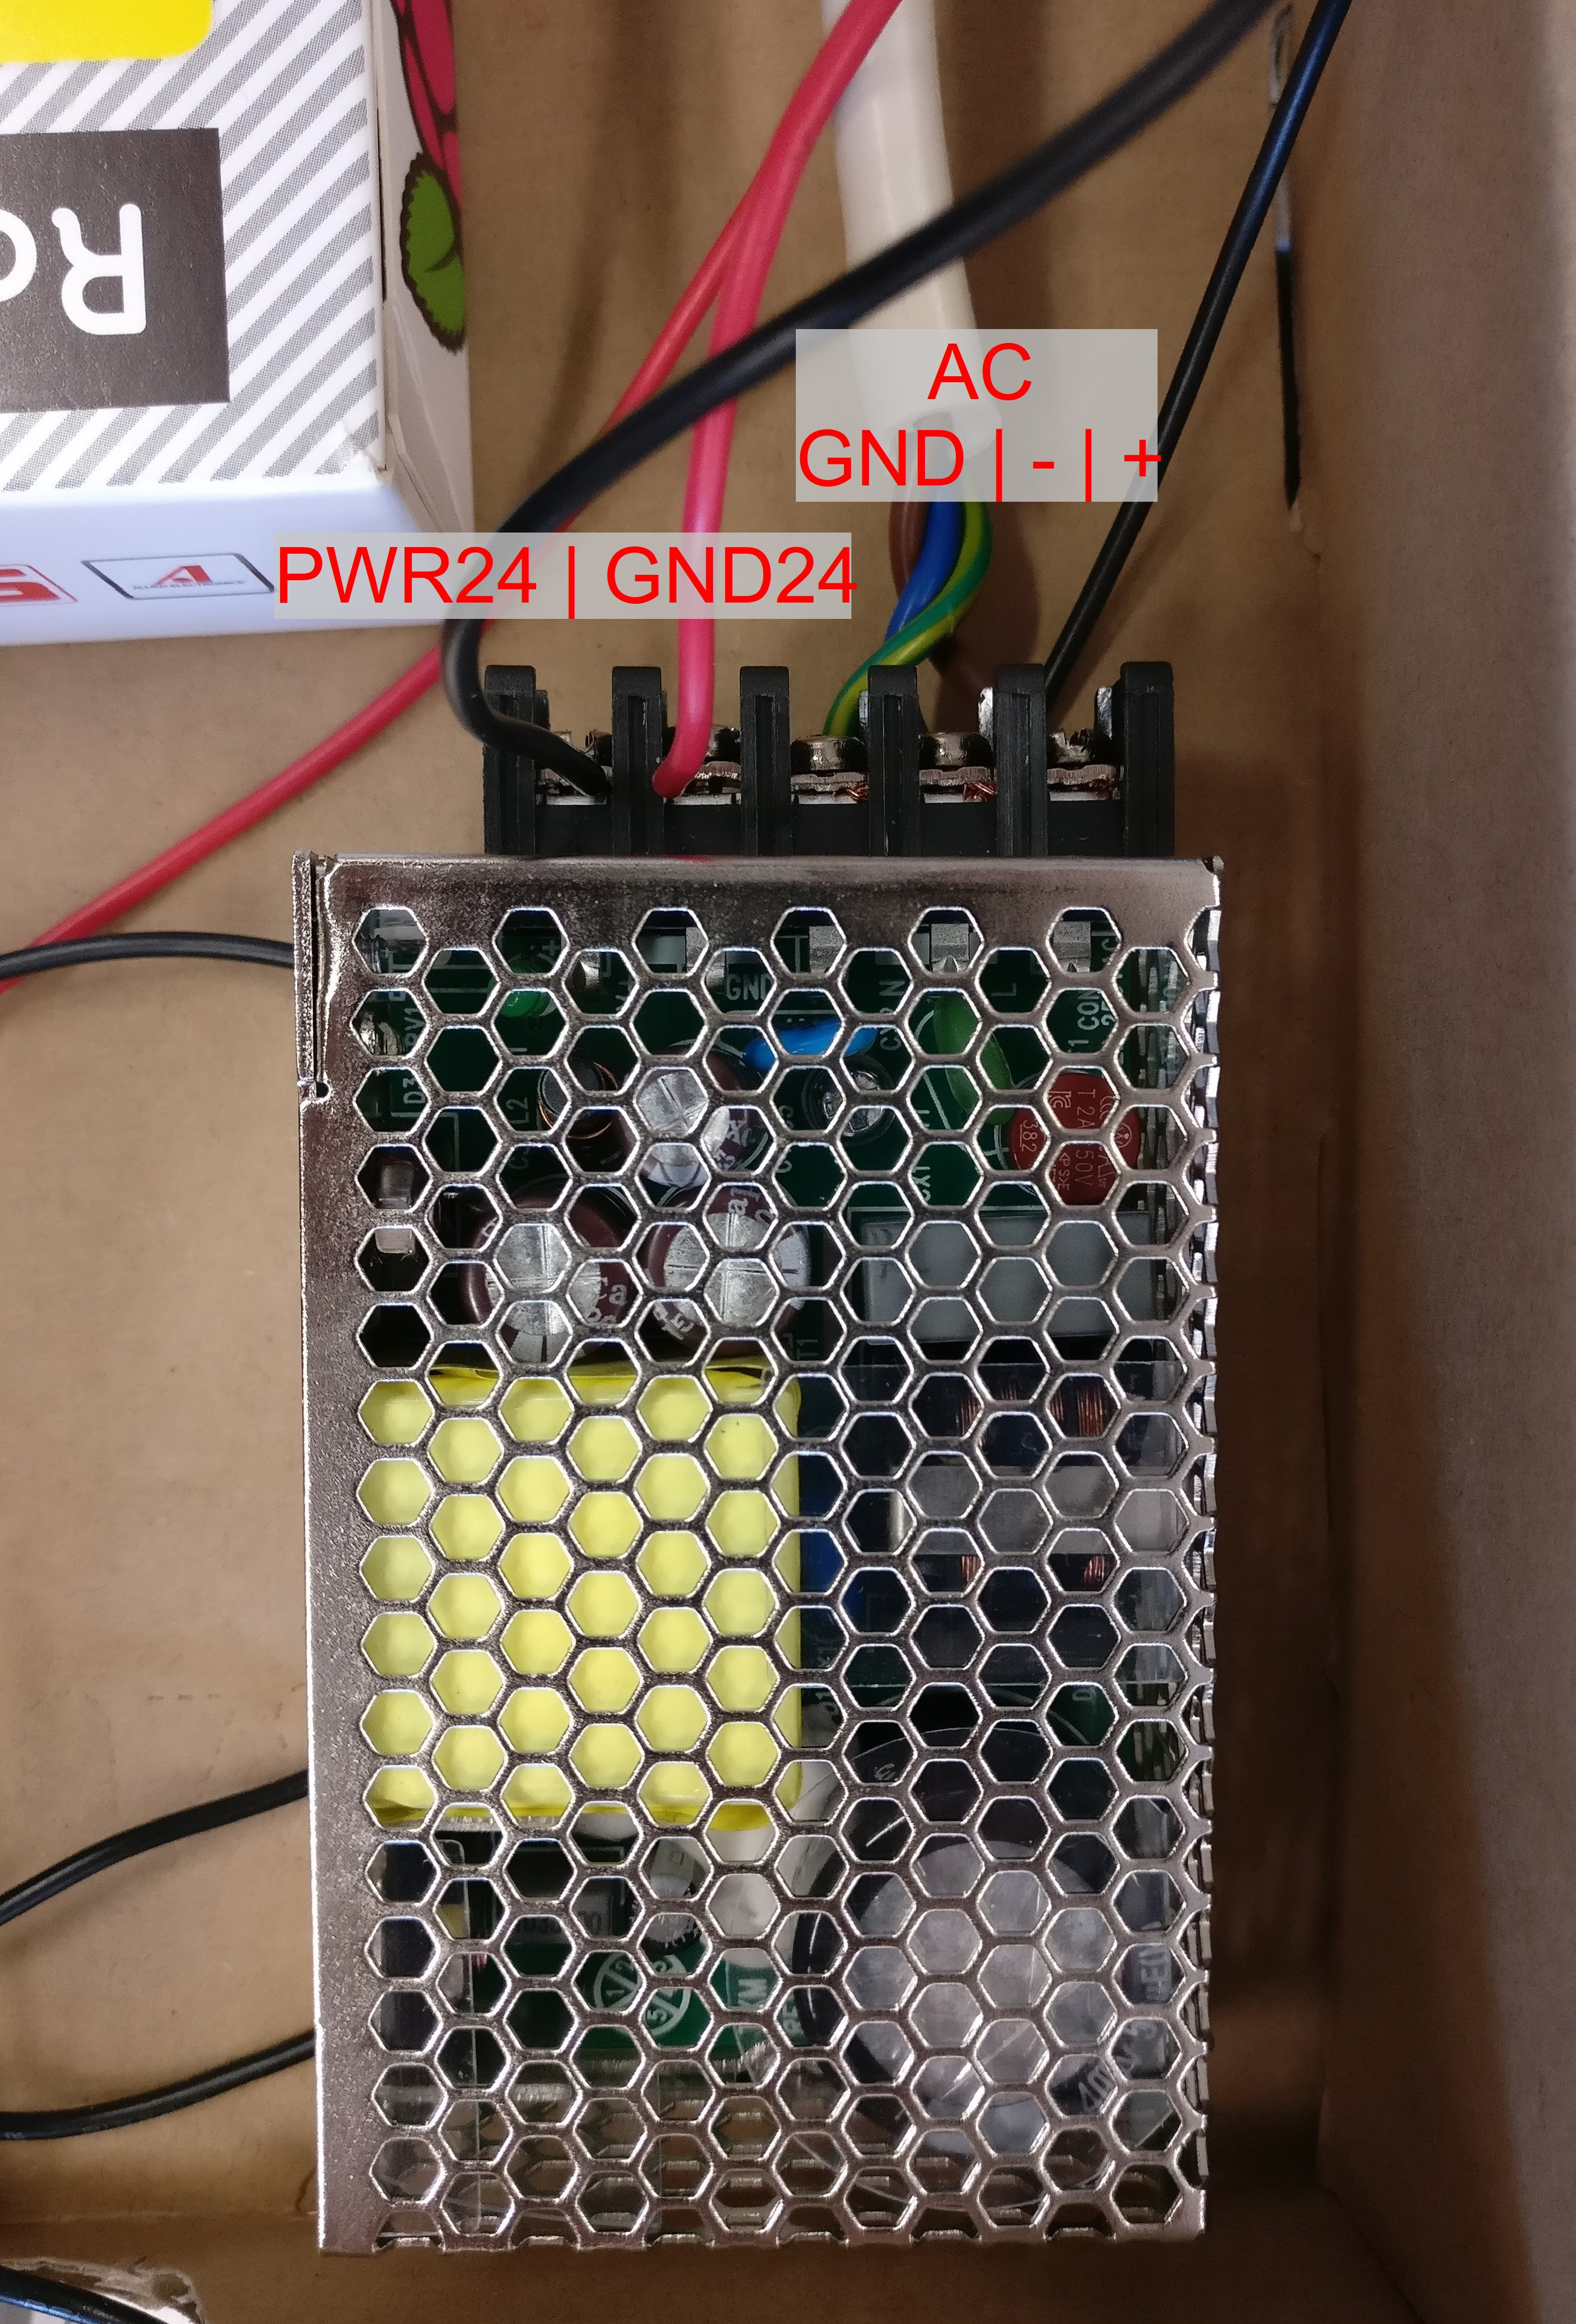
\includegraphics[width=0.7\linewidth]{ph_power24}
	\caption{24 VDC power supply.}
	\label{fig:ph_power24}
\end{figure}

\subsection{Display subsystem}
This subsystem is responsible for giving feedback to the user about the status of important signals in the different subsystems. For now, the only indicators we use are LEDs, which are:
\begin{enumerate}
	\item Valve P2 status
	\item Valve P4 status
	\item RPi server status
\end{enumerate}
All of the LEDs are connected in a circuit that is simplified in \cref{fig:led_circuit}. One yellow LED connects S1 to GND and another connects S2 to GND (see \cref{fig:ph_actuation}). Since these poles have a voltage of 24V, the resistors were calculated to be of 1500\Omega.

A red LED, is connected on the RPi's GPIO on the pin GPIO07 (3.3V, \cref{fig:rpi2_gpio}) with a 100\Omega\ resistor.


\begin{figure}
	\centering
	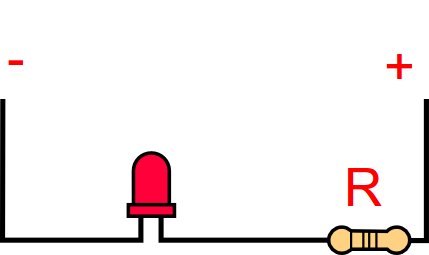
\includegraphics[width=0.4\linewidth]{led_circuit}
	\caption{Simplified circuit diagram used to power an LED.}
	\label{fig:led_circuit}
\end{figure}


\subsection{Full Setup}\label{sub:hardware:full}
Schematically, the whole system is represented in \cref{fig:subsystem_full}.
\begin{figure}[H]
	\centering
	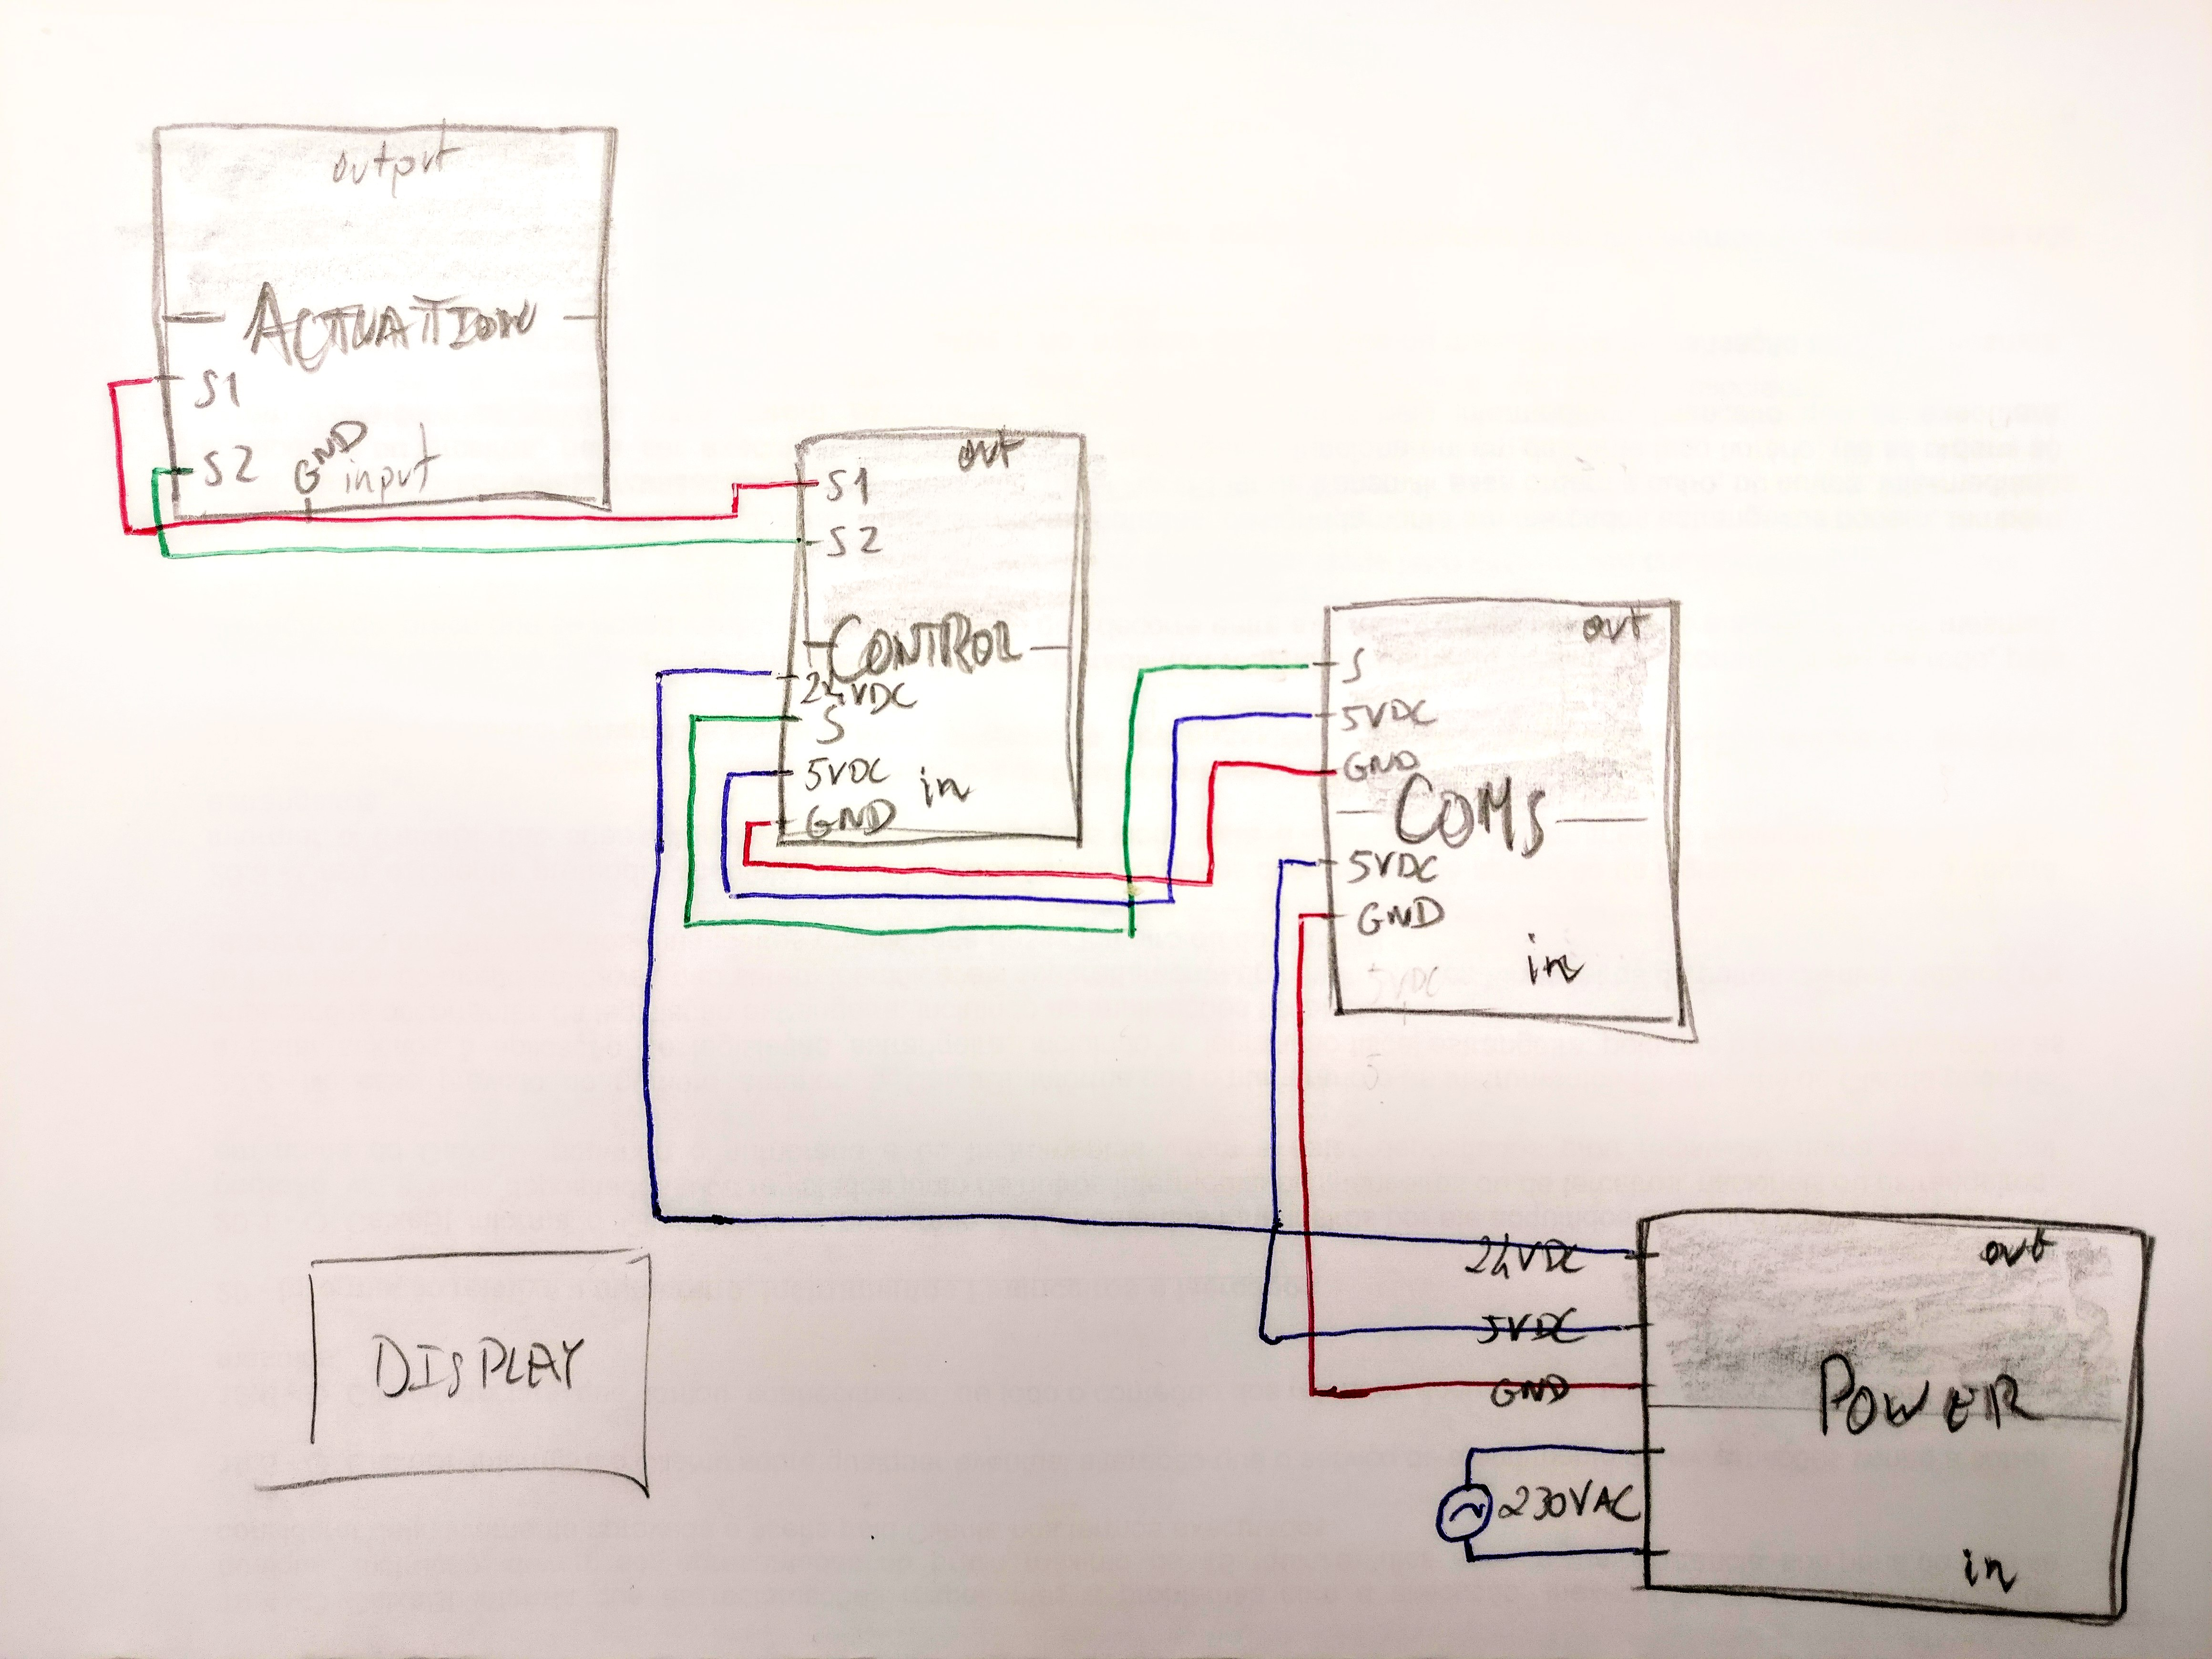
\includegraphics[width=1.0\linewidth]{subsystems_0}
	\caption{Subsystems' interactions.}
	\label{fig:subsystem_full}
\end{figure}



\section{Software}
\subsection{Operating System and Remote Access}
\marginlabel{OS Configuration}The Raspberry Pi is running a light version of Raspbian, Raspbian Jessie Lite\footnotemark. This image does not have desktop environment, so all the configuration has to be done over a terminal. Configuration steps:
\footnote{https://www.raspberrypi.org/downloads/raspbian/}
\begin{enumerate}
	\item Install OS image on the RPi's SD card
	\item Connect a keyboard, Wi-fi adapter and screen to the RPi
	\item Log into the OS with root user (pi)
	
	User name: \emph{pi}
	
	Password: \emph{raspberry}
	\item Run {\tt sudo raspi-config}
	
	Change the keyboard layout to \emph{Portuguese} (all default) 
	
	Enable SSH
	\item Set network settings, both for wi-fi and Ethernet
	\item Install {\tt git}:
	
	\begin{verbatim}sudo apt-get update
	sudo apt-get install git
	\end{verbatim}
	
\end{enumerate}
At this point, the RPi is ready to run Python 2 code. All the following configuration can be done remotely.

We can access the RPi mainframe from another computer -- preferably Linux or Windows with Putty -- over the SSH protocol using the command:

\begin{verbatim}
	ssh pi@RPI_IP_ADDRESS -p RPI_SSH_PORT
\end{verbatim}
\seealso{See \cref{sub:network_conf}}where {\tt RPI\_PI\_ADDRESS} is the IP address of the RPi and {\tt RPI\_SSH\_PORT} is the SSH port allocated to the RPi (default: 20). There should be a SSH port for each of the devices in the local network, see \cref{sub:network_conf}.

If the SSH connection was successful, you can manage the Pi. The first step is creating a known directory where to put the code into. Use the following code:

\begin{verbatim}
	mkdir /python/socket_server
\end{verbatim}
where you should replace {\tt socket\_server} by another name, if your following this documentation for another purpose.

\subsubsection{Uploading or updating the code on the Pi}
On the Pi, Python code is saved below the folder {\tt python} on the home directory:
\begin{verbatim} ~/python \end{verbatim}
With individual code packages on the directories below:
\begin{verbatim}
~/python/socket_server
~/python/code_package_1
~/python/code_package_2
~/python/code_package_3
~/python/...
\end{verbatim}

\marginlabel{Copying files remotely} It is possible to copy the code remotely with the {\tt scp} command. From your origin computer, run in one line:
\begin{verbatim}
	scp -P RPI_SSH_PORT pi@RPI_IP_ADDRESS:~/python/code_package_x/FILE.py
	/your/local/directory/FILE.py
\end{verbatim}
which copies the {\tt FILE.py} to the specified{\tt ~/python/code\_package\_x directory}. \attention If there's already a file there with the same name, it will be overwritten without warning.

\marginlabel{From git}Alternatively, you can download code from a git repository\footnotemark. You just need to run the command:

\begin{verbatim} git clone https://github.com/MiguelSimao/RPI_Control.git
~/python/socket_server
\end{verbatim}
which will copy the files inside {\tt RPI\_Control.git} to the \url{~/python/socket\_server} directory.

\footnotetext{The main author's git repository (master branch) can be found on: \\ https://github.com/MiguelSimao/RPI\_Control.git}

\subsubsection{Running a script automatically after boot}
For example, the socket server should run automatically after the OS boots. To do so, you need to follow two steps:
\begin{enumerate}
	\item
	Create a launcher script
	\item
	Add that script to {\tt crontab}
\end{enumerate}
The launcher script can be created in the home directory:
\begin{verbatim}
	nano launcher.sh
\end{verbatim}
In this file, you need to write the following code:
\begin{verbatim}
#!/bin/sh
# launcher.sh

cd /home/pi/python/socket_server
sudo python echo_server.py
\end{verbatim}
{\tt nano} is a command-line text editor, {\tt /home/pi/python/socket\_server} is the directory of the Python script and {\tt echo\_server.py} is the Python script you want to run. You can save and close the file by pressing {\tt Ctrl+X}, followed by {\tt Y} and {\tt return} (Enter). 

After that you need to make the file executable. You do so by running the following command:
\begin{verbatim} chmod 755 launcher.sh \end{verbatim}
At this stage, you can test the launcher and script by running:
\begin{verbatim} sh launcher.sh \end{verbatim}
Please note that if you need to edit the launcher file, you need to turn it back into a writable file using:
\begin{verbatim} chmod u+w launcher.sh \end{verbatim} 

The final step is writing a {\tt crontab} entry to run this script after booting. Edit the {\tt crontab} configuration by running:
\begin{verbatim} sudo crontab -e \end{verbatim}
and add the following line at the end of the file:
\begin{verbatim} @reboot sh /home/pi/bbt/launcher.sh & \end{verbatim}

This way, the RPi should be booting as usual and you should be able to {\tt SSH} into it and do whatever management you need to do, while it is also running the server.


\subsection{Socket Server}\label{sub:socket_server}
The code running the server on the RPi is on the file {\tt echo\_server.py}. This is a multi-thread server that allows several clients to be connected at the same time. The main thread loops listening for connections. The client threads -- defined by {\tt clientthread} -- reads messages from the clients and translates them into the target GPIO header configuration (pulls pins high or low as needed).

\marginlabel{Port: 1080}As is, this socket server works on the TCP channel and the port is the 1080. For the IP address, check \cref{sub:network_conf}.


\subsection{Network Configuration}\label{sub:network_conf}
The network has to be configured so that devices on the network can find the RPi. For wi-fi connections, the RPi needs to have a static IP address configured so that it can be found in the local network. To do so, follow the steps:
\begin{enumerate}
	\item
	Connect any computer to the wi-fi network (ColRobot)
	\item
	Access the router's main page at {\tt 192.168.1.1} \\
	\emph{Ask one of the lab's researchers for the credentials.}
	\item
	Go to {\tt IP \& MAC Binding / Binding Settings}
	\item
	Add your device by MAC set its IP to {\tt 192.168.1.199} or lower \\
	The attributed IPs start at .199 and decrease for each added device (.198, .197, ...)
\end{enumerate}
\marginlabel{IP Address}At this point, you can access the RPi in the wi-fi network (not ethernet) using the static IP you set before.

\subsubsection{Wired Connection}
\marginlabel{Local IP: 172.31.1.1}
Currently, the RPi's IP address the robot's LAN is 172.31.1.1. If you would like to change or add a new device, do not define an IP that's already in use. You may lose remote access to the RPi!

To set up the local wired connection, you just need to edit the file {\tt /etc/network/interfaces} by running the line:
\begin{verbatim}sudo nano /etc/network/interfaces \end{verbatim}
to edit the file. Comment out with a '\#' the line that starts with -- {\tt iface eth0 inet *} -- and add the following lines to the end:
\begin{verbatim}
# The loopback interface
auto lo
iface lo inet loopback
auto eth0
iface eth0 inet static
# YOUR STATIC IP:
address 172.31.1.1
netmask 255.255.255.0
\end{verbatim}
\marginlabel{Be careful, do not set up two machines with the same static IP!}
Then press {\tt Ctrl+X}, then {\tt Y} and return (Enter) to save the edited file. After restarting the connection (you can reboot the RPi with a {\tt sudo reboot}), you should be able to connect to the RPi through that static IP address if you're in the same local network. You may have to change your computer's IP address to one of the same range (172.31.1.1-255) to be able to establish a connection.

\subsubsection{Remote Communications}
As remote, we mean connecting through the network to which the wi-fi router is connected. The router has a static IP address on the department's network -- {\tt ROUTER\_IP} -- and you can access the router through that IP from any computer connected to any of the Ethernet ports on the lab.
If you want to send a command from a remote location (e.g., computer connected to the lab network, outside of the wi-fi network), first you need to connect to the router through {\tt ROUTER\_IP}. The router then decides the device it will send a packet to. \marginlabel{Port Forwarding}This is done by port forwarding. 

By default, you can connect remotely to the RPi by SSH using port 22 and TCP using port 1080. If more computers are on the same network (e.g., other RPi), you need to configure them to have non-default ports,  often on the range between 1024 and 65535. To do so, follow these steps:
\begin{enumerate}
	\item
	Access the router's main page at {\tt 192.168.1.1} or {\tt ROUTER\_IP}  \\
	\emph{Ask one of the lab's researchers for the credentials.}
	\item
	Go to {\tt Forwarding / Virtual Servers}
	\item
	Add new entry by setting the port you want (Service port) and the static IP address you set for the corresponding device previously.
\end{enumerate}



\end{document}